%% $Id: projplan.tex,v 1.5 1999/12/17 16:48:09 matt Exp $

\chapter{Project Plan}
In order for the project to be a success it must be ensured that it finishes on time and that we have allocated enough time and resources for each task.

\section{Timeline}
The project has been broken up into individual tasks that need to be completed.  A Gantt chart representing these tasks is shown in Figure \ref{gantt}.  The other members of Etherworks have been included in this plan, however their actual work should not be considered part of the project, and hence is not shown to any detail.


\begin{figure}[!ht]
\begin{center}
\epsfig{file=gantt.eps,angle=-90,width=10cm} 
\end{center}
\label{gantt}
\caption{Project Gantt Chart}
\end{figure}

\subsection{Task list}

\begin{itemize}
\item Customer Requirements\\{\em 1999.Oct.04 - 1999.Oct.15; assigned to Matt Hamilton}

{\em The other members of Etherworks and the Open Source community as a whole were asked for what they thought was required of the service.}
\item Initial Specification\\{\em 1999.Oct.18 - 1999.Oct.22; assigned to Matt Hamilton}

{\em An overall structure for the archive was devised and the principle components marked out.  This will later be expanded into the Technical Specification}
\item Prototype\\{\em 1999.Nov.01 - 1999.Nov.26; assigned to Matt Hamilton}

{\em A prototype was built to test if the idea is feasible.  The prototype was written in C and specifically tested the speed and scalability of the compression algorithms found in \cite{wmb:mg}.}
\item Risk Analysis\\{\em 1999.Dec.10 - 1999.Dec.16; assigned to Matt Hamilton}

{\em The main risks that could cause the project to fail or not be completed on time were predicted. Their probability of occurrence and consequences as well as what could be done to reduce this risk were estimated.}
\item Technical Specification\\{\em 2000.Jan.11 - 2000.Jan.21; assigned to Matt Hamilton}

{\em The Technical Specification will contain the exact design of the backend components for the archive.   The coding of the end product will be based upon this document and will be useful for anybody else wanting to modify the code.}
\item Design DB Structure\\{\em 2000.Jan.25 - 2000.Jan.27; assigned to Matt Hamilton}

{\em The messages will be stored in a database, the structure of which needs to be designed.  The database will also hold information such as user preferences and administravia.}
\item Coding Parser\\{\em 2000.Jan.28 - 2000.Feb.16; assigned to Matt Hamilton}

{\em The parser that decodes messages and inserts the into the database will be coded}
\item Test Parser\\{\em 2000.Feb.17 - 2000.Feb.23; assigned to Matt Hamilton}

{\em Testing of the parser will involve subscribing to many mailing lists and testing to see if the parser can parse all of the messages.}
\item Code Indexer\\{\em 2000.Feb.24 - 2000.Mar.14; assigned to Matt Hamilton}

{\em The indexer that fetches messages from the database and produces the index files used by the Query Server will be written.}
\item Test Indexer\\{\em 2000.Mar.15 - 2000.Mar.21; assigned to Matt Hamilton}

{\em The indexer will be tested and profiled to make sure it is fast enough.  It is expected that there will be quite a few refinements of the code to try and squeeze as much speed as possible out of the indexer.  This task will also involve coding a decoder to make sure that the indexes produced are valid.}
\item Code Query Server\\{\em 2000.Jan.28 - 2000.Apr.10; assigned to Matt Hamilton}

{\em The daemon that accepts queries from the web server will be coded.}
\item Test Query Server\\{\em 2000.Apr.11 - 2000.Apr.17; assigned to Matt Hamilton}

{\em Testing the Query Server will involve creating sample scripts to submit queries to the Query Server and time response times.}
\item Code Web Scripts\\{\em 2000.Jan.28 - 2000.May.05; assigned to Matt Hamilton}

{\em These scripts will form a library or module with functions to submit queries, and retrieve list indexes and messages.  They will be called by the web pages being designed by Chris Parsons.}
\item Test Web Scripts\\{\em 2000.May.08 - 2000.May.12; assigned to Matt Hamilton}

{\em The scripts will be tested with some simple HTML pages to make sure they work correctly.  At this point we should have all of the functionality of the archive implemented.}
\item Backend Integration Testing\\{\em 2000.May.15 - 2000.May.26; assigned to Matt Hamilton}

{\em All of the backend components will be tested together to make sure that they work correctly with each other.}
\item Thesis Writeup\\{\em 2000.Jun.06 - 2000.Jul.03; assigned to Matt Hamilton}

{\em The remaining parts of the this thesis will be written up.  Also a complete business plan will be written to project where we go from the end of the project.}
\item Design Admin Site Tools\\{\em 2000.Jan.11 - 2000.Apr.28; assigned to Tim Saigol}

{\em Tim Saigol will be designing administrative tools that will be needed for the day-to-day running of the archive once we launch.}
\item Design Web Site Graphics\\{\em 2000.Jan.11 - 2000.Apr.28; assigned to Chris Green}

{\em Chris Green will be designing the graphics for the web site and deciding the overall look and feel of the site.}
\item Design Web Site Layout\\{\em 2000.Jan.11 - 2000.Apr.28; assigned to Chris Parsons}

{\em Chris Parsons will be working on designing the final web site layout.  He will be coding the needed HTML and calling the backend scripts that will be written as part of this project.}
\item Frontend Integration Testing\\{\em 2000.May.01 - 2000.May.12; assigned to Chris Parsons}

{\em The graphics, HTML and scripts will be tested together to ensure a consistent look and feel across the site and that the site works under different web browsers and at different connection speeds.}
\item Beta Test\\{\em 2000.May.29 - 2000.Jun.02; assigned to Resource group}

{\em Selected groups of people will be asked to test the site and let us know what they think.  Any changes and improvements will be made at this time.  We will also do synthetic load benchmarks to see how the server will handle heavy loads and realistically how many concurrent users we can support.}
\item Archive Site Launch\\{\em 2000.Jun.05 - 2000.Jun.05; assigned to Resource group}

{\em Launch the site!  We will advertise the site on various other web sites and discussion forums and try and get as much interest as possible.}
\end{itemize}


\subsection{Resources and task assignment}

\subsubsection{Matt Hamilton }

\begin{supertabular}{|l|l|r|r|p{2in}|}
\hline
{\bf Start} & {\bf Finish} & {\bf Days} & {\bf Done} & {\bf Task} \\
\hline
 1999.Oct.04 & 1999.Oct.15 & 10 & 10 & Customer Requirements \\
 1999.Oct.18 & 1999.Oct.22 & 5 & 5 & Initial Specification \\
 1999.Nov.01 & 1999.Nov.26 & 20 & 20 & Prototype \\
 1999.Dec.10 & 1999.Dec.16 & 5 & 5 & Risk Analysis \\
 1999.Dec.21 & 2000.Jan.05 & 12 & 0 & Vacation \\
 2000.Jan.11 & 2000.Jan.21 & 9 & 0 & Technical Specification \\
 2000.Jan.25 & 2000.Jan.27 & 3 & 0 & Design DB Structure \\
 2000.Jan.28 & 2000.Feb.16 & 14 & 0 & Coding Parser \\
 2000.Feb.17 & 2000.Feb.23 & 5 & 0 & Test Parser \\
 2000.Feb.24 & 2000.Mar.14 & 14 & 0 & Code Indexer \\
 2000.Mar.15 & 2000.Mar.21 & 5 & 0 & Test Indexer \\
 2000.Jan.28 & 2000.Apr.10 & 14 & 0 & Code Query Server \\
 2000.Apr.11 & 2000.Apr.17 & 5 & 0 & Test Query Server \\
 2000.Jan.28 & 2000.May.05 & 14 & 0 & Code Web Scripts \\
 2000.May.08 & 2000.May.12 & 5 & 0 & Test Web Scripts \\
 2000.May.15 & 2000.May.26 & 10 & 0 & Backend Integration Testing \\
 2000.Jun.06 & 2000.Jul.03 & 20 & 0 & Thesis Writeup \\
\hline
\multicolumn{5}{l}{\bf Total: 158 days scheduled, 40 days completed.}\\
\end{supertabular}


\subsubsection{Tim Saigol }

\begin{supertabular}{|l|l|r|r|p{2in}|}
\hline
{\bf Start} & {\bf Finish} & {\bf Days} & {\bf Done} & {\bf Task} \\
\hline
 1999.Dec.21 & 2000.Jan.05 & 12 & 0 & Vacation \\
 2000.Jan.11 & 2000.Apr.28 & 79 & 0 & Design Admin Site Tools \\
\hline
\multicolumn{5}{l}{\bf Total: 79 days scheduled, 0 days completed.}\\
\end{supertabular}


\subsubsection{Chris Green }

\begin{supertabular}{|l|l|r|r|p{2in}|}
\hline
{\bf Start} & {\bf Finish} & {\bf Days} & {\bf Done} & {\bf Task} \\
\hline
 1999.Dec.21 & 2000.Jan.05 & 12 & 0 & Vacation \\
 2000.Jan.11 & 2000.Apr.28 & 79 & 0 & Design Web Site Graphics \\
\hline
\multicolumn{5}{l}{\bf Total: 79 days scheduled, 0 days completed.}\\
\end{supertabular}

\pagebreak
\subsubsection{Chris Parsons }

\begin{supertabular}{|l|l|r|r|p{2in}|}
\hline
{\bf Start} & {\bf Finish} & {\bf Days} & {\bf Done} & {\bf Task} \\
\hline
 1999.Dec.21 & 2000.Jan.05 & 12 & 0 & Vacation \\
 2000.Jan.11 & 2000.Apr.28 & 79 & 0 & Design Web Site Layout \\
 2000.May.01 & 2000.May.12 & 10 & 0 & Frontend Integration Testing \\
\hline
\multicolumn{5}{l}{\bf Total: 89 days scheduled, 0 days completed.}\\
\end{supertabular}


\subsubsection{Chris Green, Chris Parsons, Tim Saigol, Matt Hamilton }

\begin{supertabular}{|l|l|r|r|p{2in}|}
\hline
{\bf Start} & {\bf Finish} & {\bf Days} & {\bf Done} & {\bf Task} \\
\hline
 2000.May.29 & 2000.Jun.02 & 5 & 0 & Beta Test \\
 2000.Jun.05 & 2000.Jun.05 & 1 & 0 & Archive Site Launch \\
\hline
\multicolumn{5}{l}{\bf Total: 6 days scheduled, 0 days completed.}\\
\end{supertabular}




\section{Resources}

\subsection{Server}\label{serverspecs}
A server has been provided by Etherworks for the development and hosting of the archive.  The Department of Computer Science has kindly allowed the server to be connected to their network, where is can stay during the development stage of the project, however it must be moved for the launch of the site.


\begin{table}[!ht]
\begin{center}
\begin{tabular}{|l|l|}
\hline
Memory          & 300MB \\
\hline
Processors      & 2 x 300Mhz Intel Pentium II \\
\hline
Storage         & 4 x 4GB Wide SCSI Hard Disks \\
                & DPT RAID 5 Controller with 8MB cache \\
\hline
OS              & FreeBSD 3.4 \\
\hline
\end{tabular}
\caption{Server Specification}
\end{center}
\end{table}

% LocalWords:  Timeline ht gantt eps MB Mhz Pentium GB DPT
